

\subsubsection{KW40: 04.10.2021 bis 10.10.2021}
\begin{quote}
	\subsubsection*{Arbeit in der Schule}
	
	
	Besprechung mit Herrn Rusch:
	
	Wir haben gemeinsam mit Herrn Rusch das Programm Latex auf unserer
	Virtual Machine installiert. Anschließend haben wir unser Repository, die wir im Gitlab erstellt haben, in unserem PC geklont.
	
	Dies wurde mit dem folgenden Befehl realisiert: git clone {[}url-vom
	Projekt{]}.
	
	\subparagraph{\texorpdfstring{Daten uplod:
	}{Daten uplod: }}
	
	Um Daten auf GitLab hochzuladen, werden folgende Befehle ausgeführt:
	
	Zuerst muss im Terminal auf unser Repository-Ordner navigiert werden:
	
	\texttt{ls\ -l} : Inhalt des Verzeichnis
	
	\texttt{cd\ Verzeichnisname} : in den Ordner wechseln
	
	\texttt{git\ status} : Abfrage ob im lokalen Repository etwas verändert
	wurde
	
	\texttt{git\ add}. : eine Änderung aus dem Arbeitsverzeichnis wir zur
	Staging-Umgebung hinzugefügt
	
	\texttt{git\ commit\ -am\ "name"} : Der Befehl committet den Snapshot im
	Staging-Bereich in die Projekt-Historie
	
	\texttt{git\ push} : Änderung werden hochgeladen
	
	\subparagraph{Daten download:}
	
	hier muss wieder auf unseren Repository-Ordner navigiert werden.
	
	\texttt{git\ pull} : Inhalte vom Repository herunterladen um das lokale
	Repository zu aktualisieren
	
	Danach hat uns Herr Rusch eine Einführung zum Programm LaTex gegeben.
	
	
	\paragraph{Arbeit außerhalb der Schule}
	
	
	Ich habe am Programm, welches für die Bewegung vom Charakter dient,
	weitergearbeitet.
	
	Es wurde ein Animator Controller erstellt, bei der 2 Zustände im State
	Machine definiert worden sind. Nachdem das Spiel gestartet wird(Entry),
	wird sofort der Zustand idle übernommen. Mit der Animation idle steht
	der Charakter ohne Bewegung. Doch wenn die Boolvariable IsWalking wahr
	wird, geht der Zustand von idle zu run, welches den Charakter in
	Bewegung setzt. Wenn die Boolvariable IsWalking wieder unwahr wird,
	kährt sie zum default state, also zum idle wieder zurück. Die
	Animationen wurden vom Character Pack: Free Sample entnommen.
	\begin{center}
		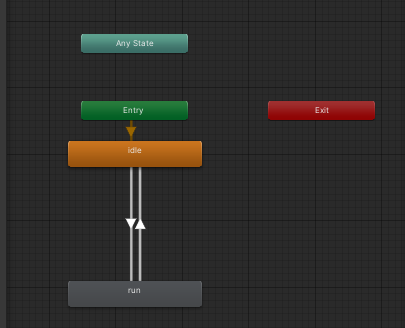
\includegraphics[frame, height=6cm]{img/SemihSoenmez_IMG/StateMachine_SS_KW41_041021.png}
	\end{center}

	Anschließend wurde der Animator Controller zum Prefab Model zugewiesen.
	
	
	\subsubsection*{Was ist geplant für die Nächste Woche}
	Es soll mit dem Character Controller Programm weitergearbeitet werden.
\end{quote}	

